\subsection{Distrución del uso de las estaciones}

En la figura \ref{fig:map_metro_stations} se visualizan las linea del metro (roja, azul marino y verde) y del metrobus (azul claro). Como se mencionó en la introducción, el sistema público de bicicletas está enfocado en disminuir la congestión del tráfico usando vías adecuadas y en puntos apropiados. Esto se ve reflejado en la figura \ref{fig:map_metro_stations}, ya que la mayoria de las estaciones se encuentran en los polígonos de intervención urbana especial (PIUE), que son áreas enfocadas al desarrollo social, medioambiental y económico\cite{poligono_2018}. Las estaciones que están fuera de los PIUE, se encuentran alrededor de las lineas del metro o en zonas en donde el transporte público es deficiente (esquina inferior izquierda). Esto puede ser debido a que fueron instaladas para suplir el uso del metro cuando no sea eficiente para el usuario.

\begin{figure}[H]
    \centering
    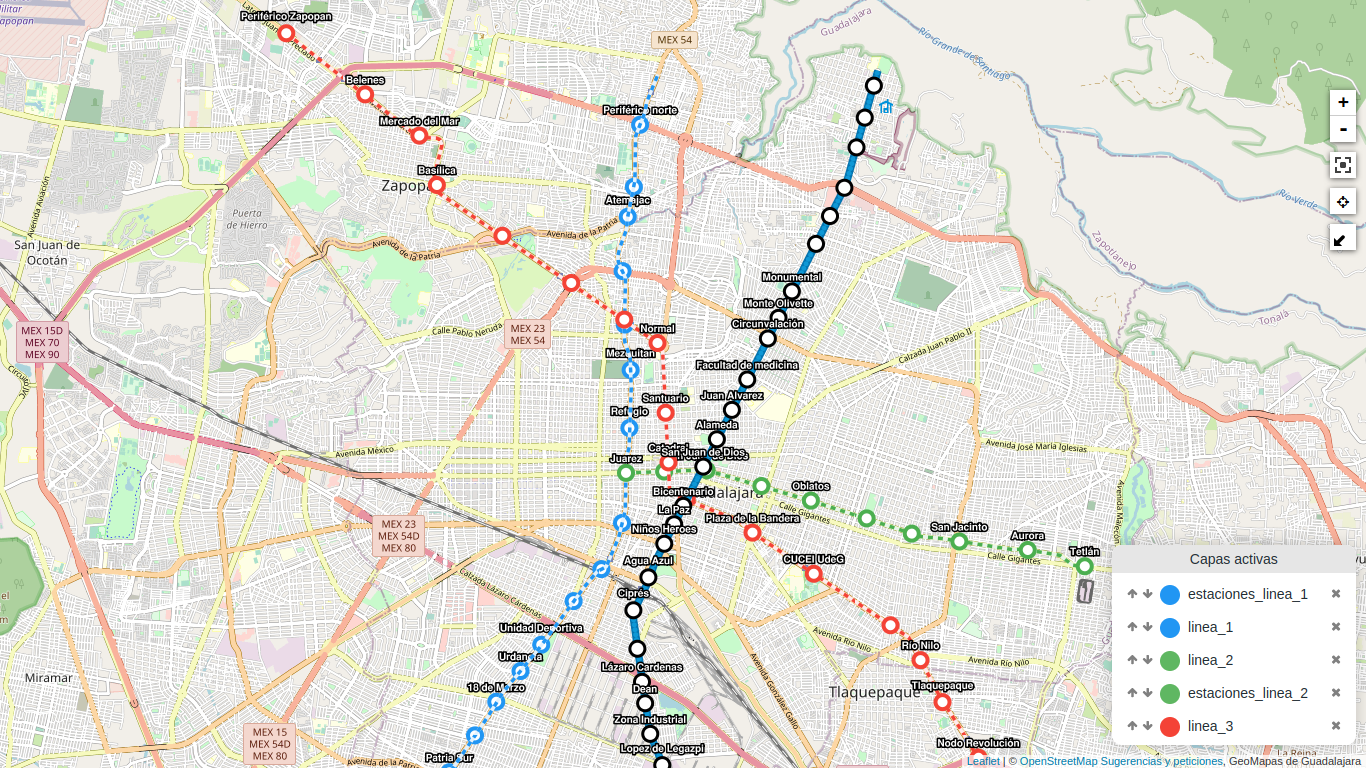
\includegraphics[width=8cm,height=5cm]{Graphics/map_with_metro_lines.png}
    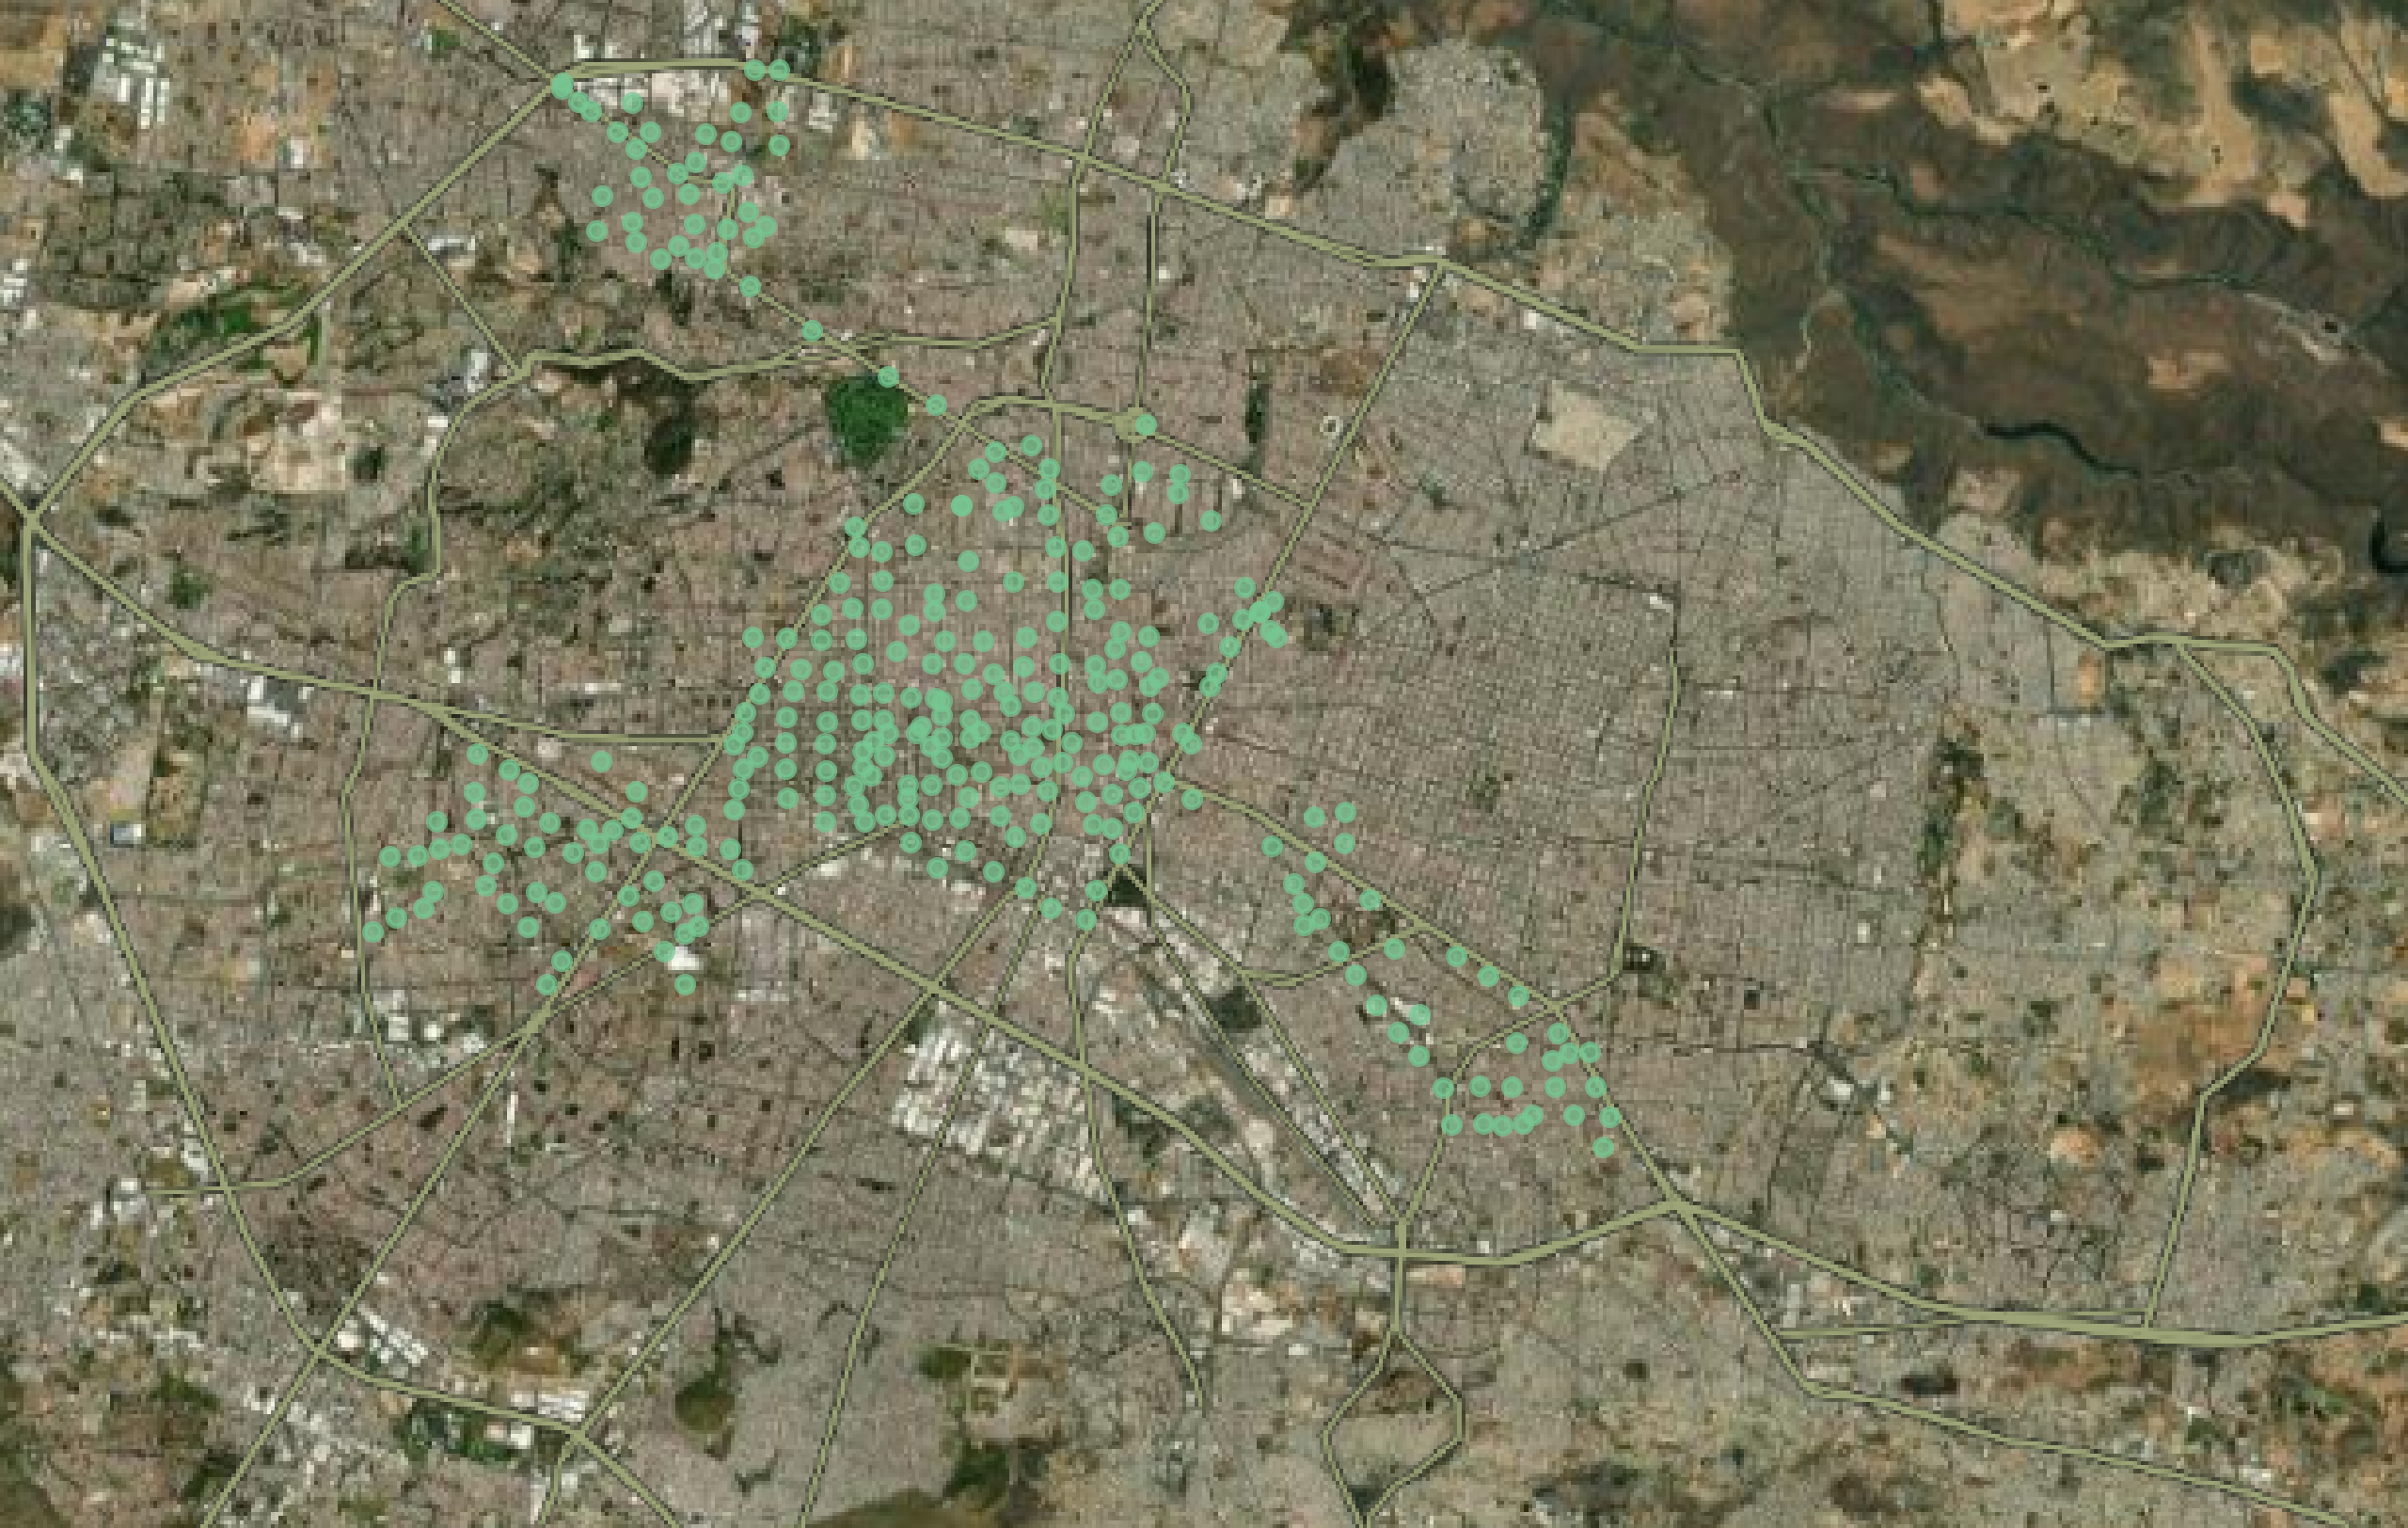
\includegraphics[width=8cm,height=5cm]{Graphics/stations.png}
    \caption{Mapa de la zona metropolitana de Guadalajara señalando las lineas del metro (izquierda) y las estaciones de MiBici (derecha).}
    \label{fig:map_metro_stations}
\end{figure}

En la figura \ref{fig:distribution_station_all_origin} se puede notar que las estaciones localizadas en PIUE son las más usadas con respecto a las estaciones que se encuentran en los límites de la zona metropolitana. En la figura \ref{fig:distribution_station_zoom_origin} se observa que las estaciones que se encuentran en la Avenida Ignación L. Vallarta y las que se encuentran en las intersecciones de las lineas de metro son las que reciben más uso por parte de los usuarios.

\begin{figure}[H]
    \centering
    \begin{subfigure}[b]{8.2cm}
        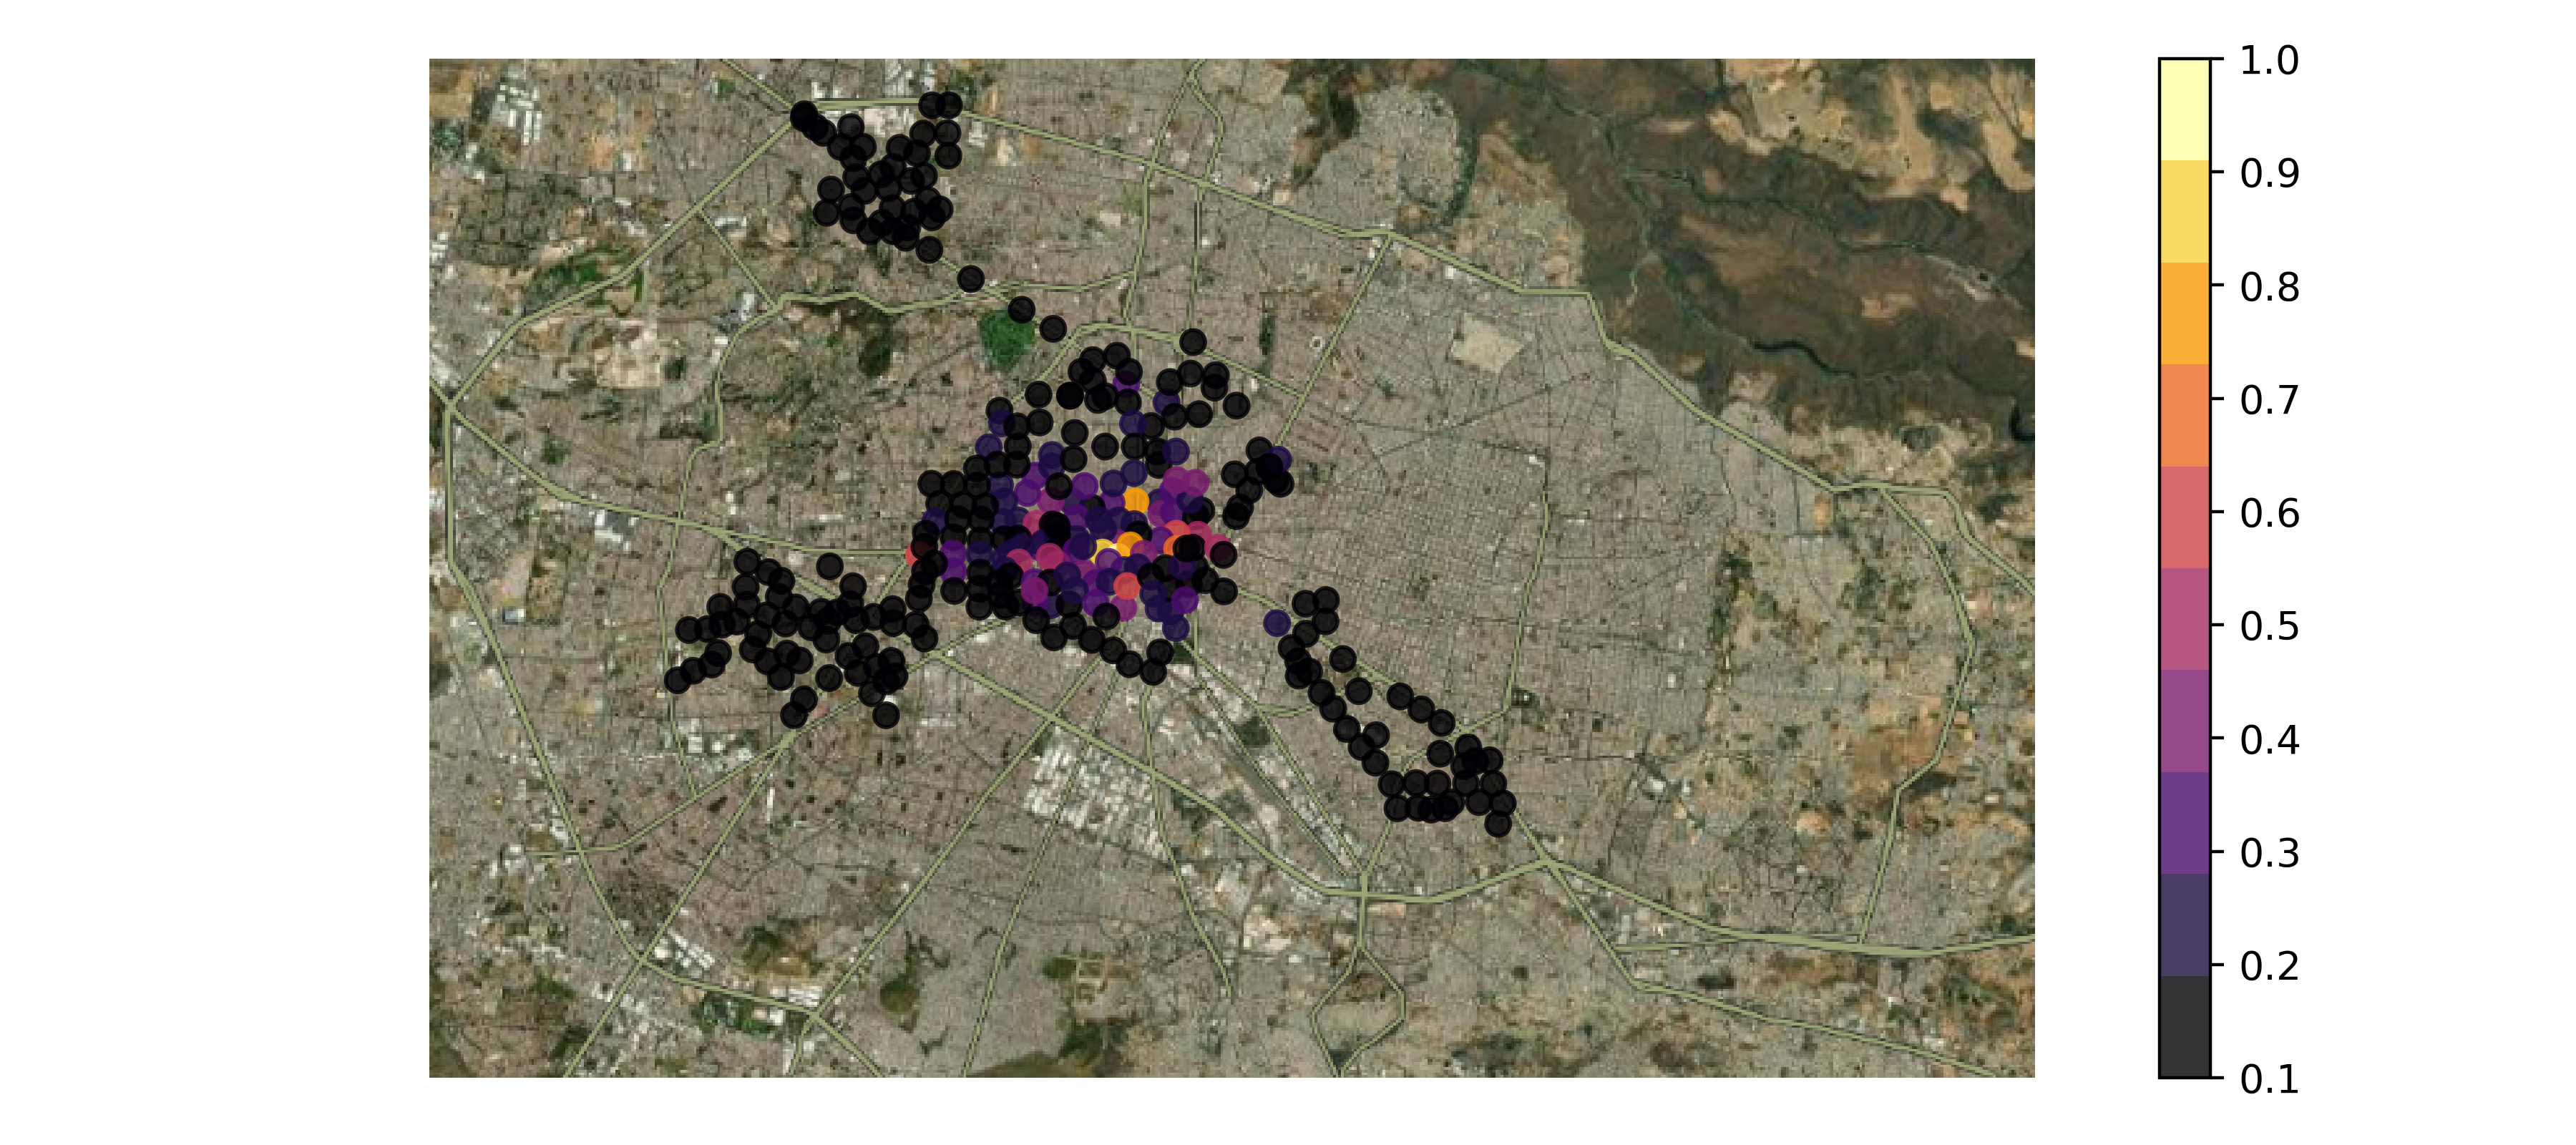
\includegraphics[width=8.2cm]{Graphics/repetition_origen.png}
        \caption{Zona metropolitana de Guadalajara.}
        \label{fig:distribution_station_all_origin}
    \end{subfigure}
    % \hspace{0.5cm}
    \begin{subfigure}[b]{8.2cm}
        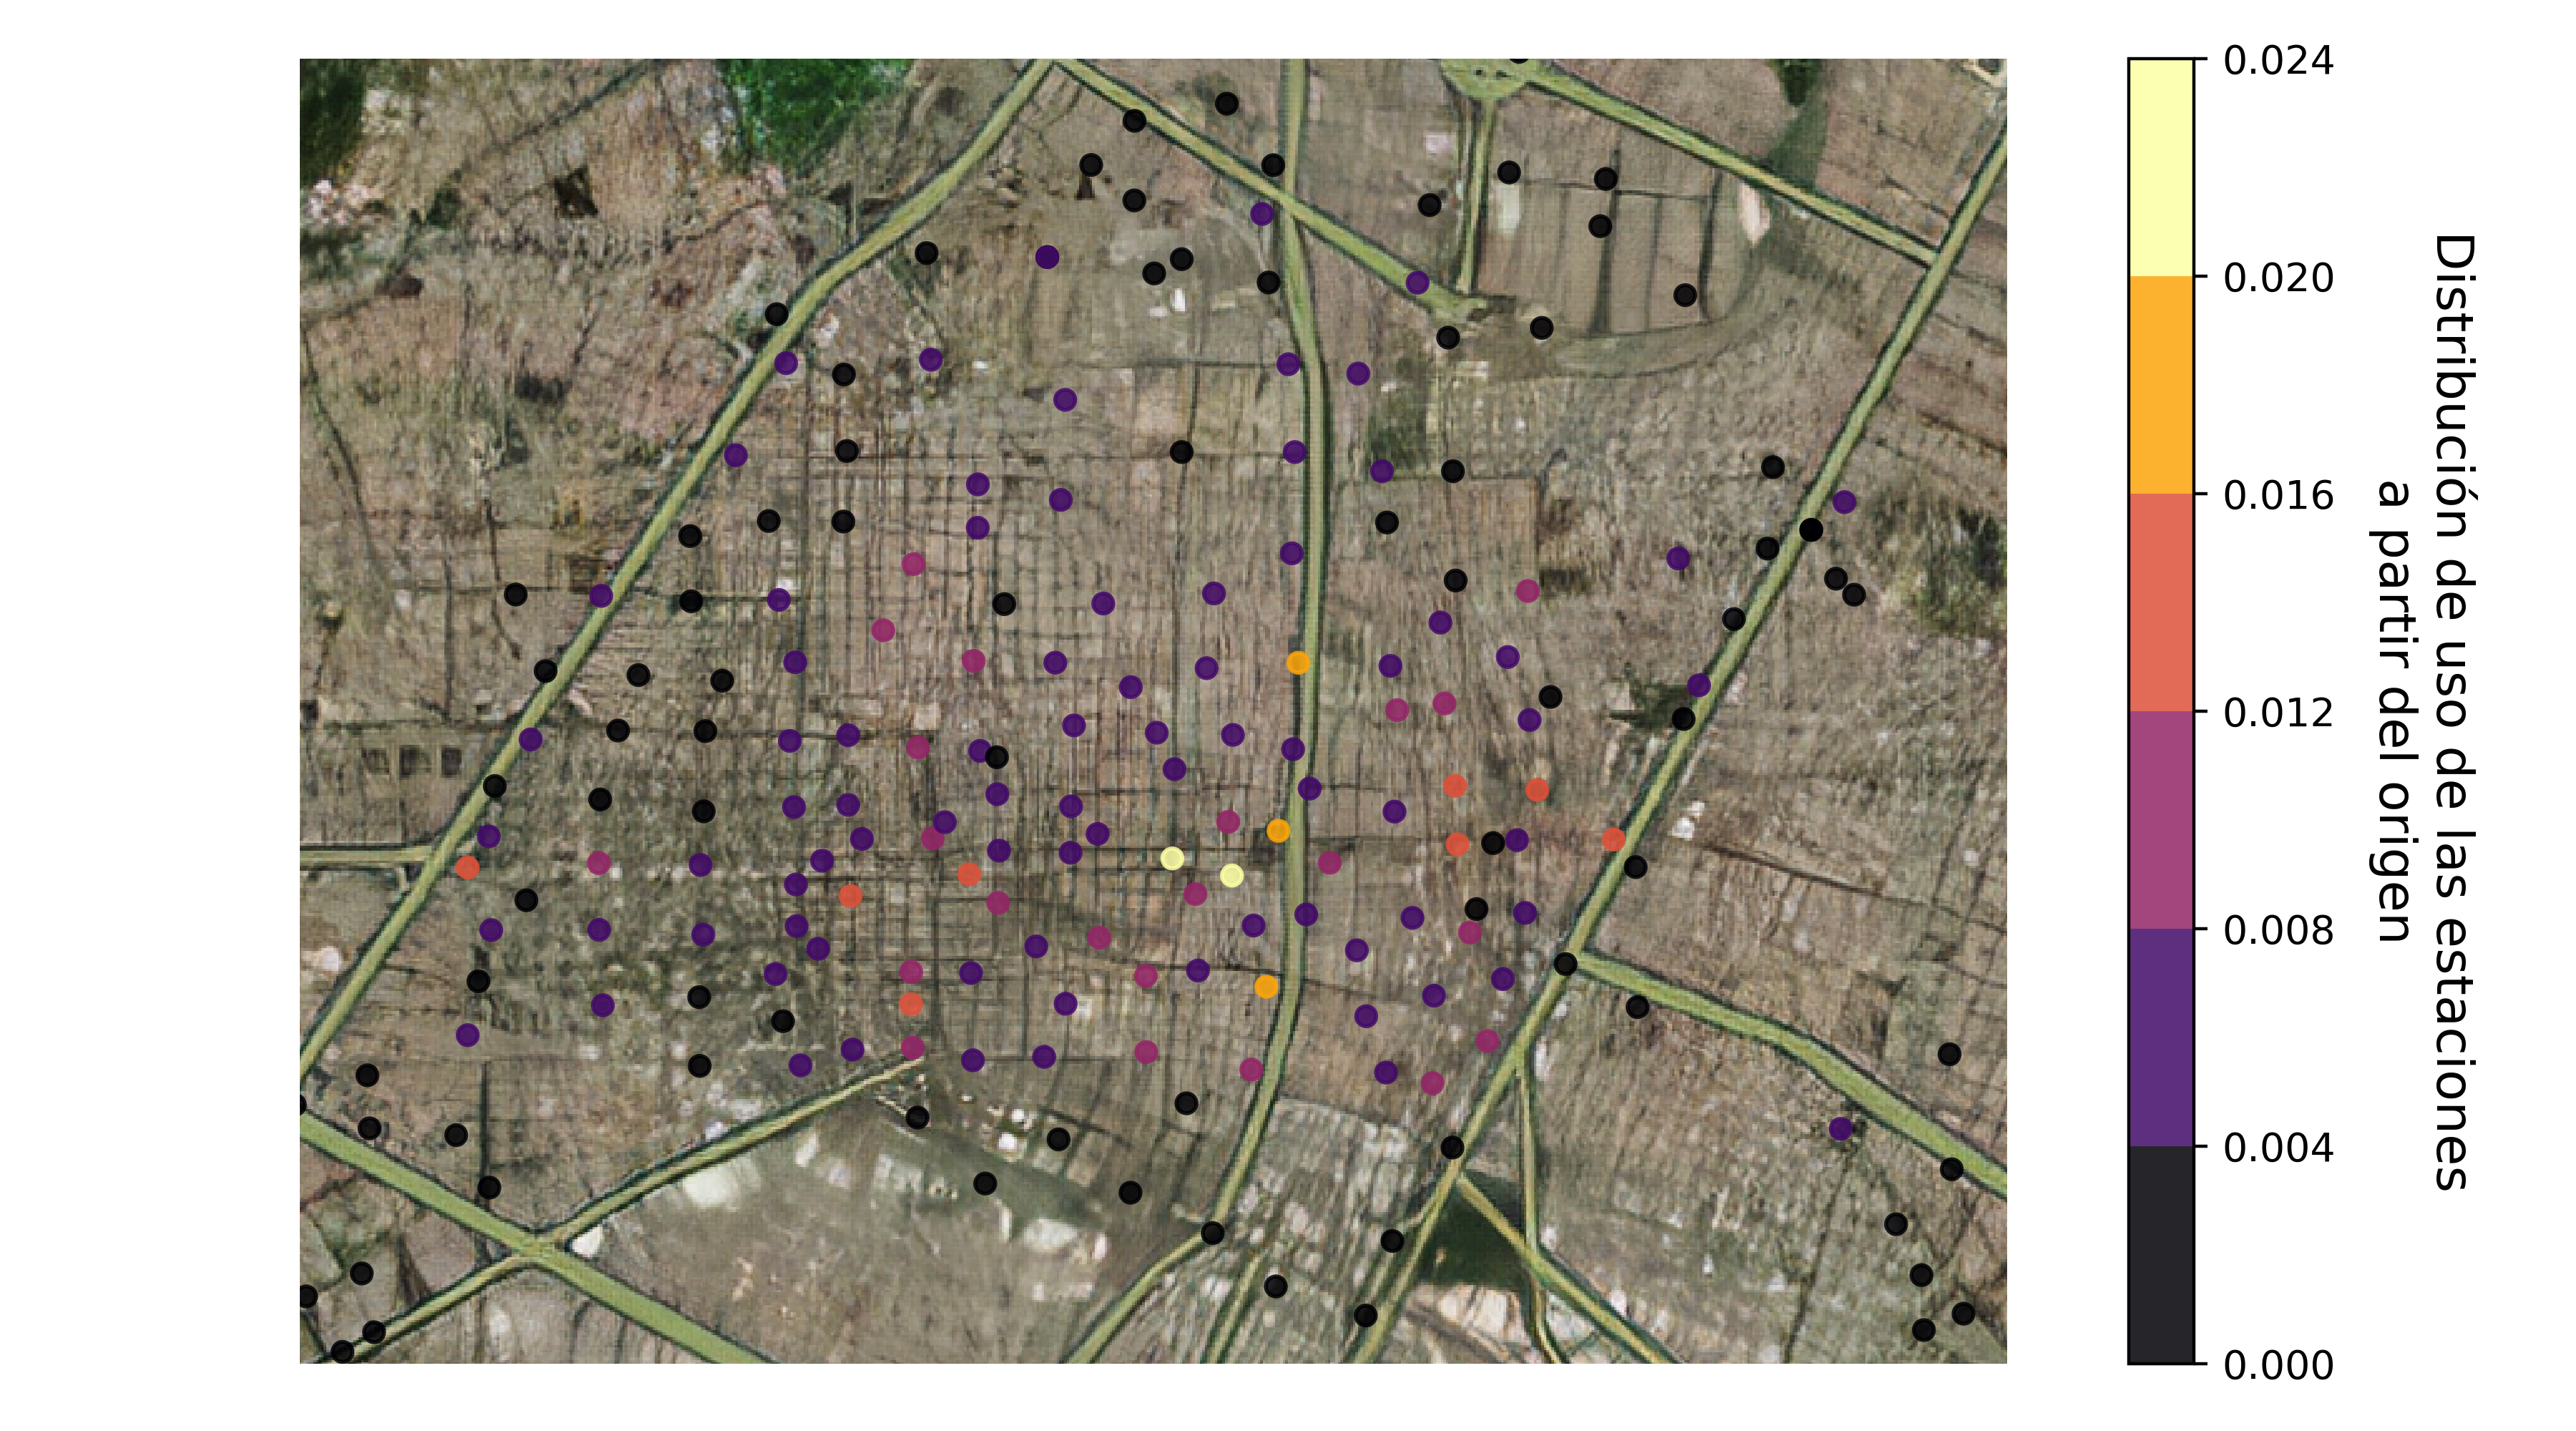
\includegraphics[width=8.2cm]{Graphics/repetition_origen_zoom.png}
        \caption{Zona de Chapultepec y Santa Tere.}
        \label{fig:distribution_station_zoom_origin}
    \end{subfigure}
    \caption{Distribución del uso de las estaciones de MiBici como punto de origen.}
    \label{fig:distribution_origin}
\end{figure}

Al considerar las estaciones que son usadas como destino del viaje se obtiene la figura \ref{fig:distribution_destiny}. Comparando las figuras \ref{fig:distribution_origin} y \ref{fig:distribution_destiny} se visualiza que las estaciones que se encuentran en las intersecciones de las lineas del metro son las más usadas. Esto puede ser un reflejo de que el servicio de bicicletas es utilizado para transportarse en distancias cortas y como auxiliar para disminuir la aglomeración de personas en el transporte público.

\begin{figure}[H]
    \centering
    \begin{subfigure}[b]{8.2cm}
        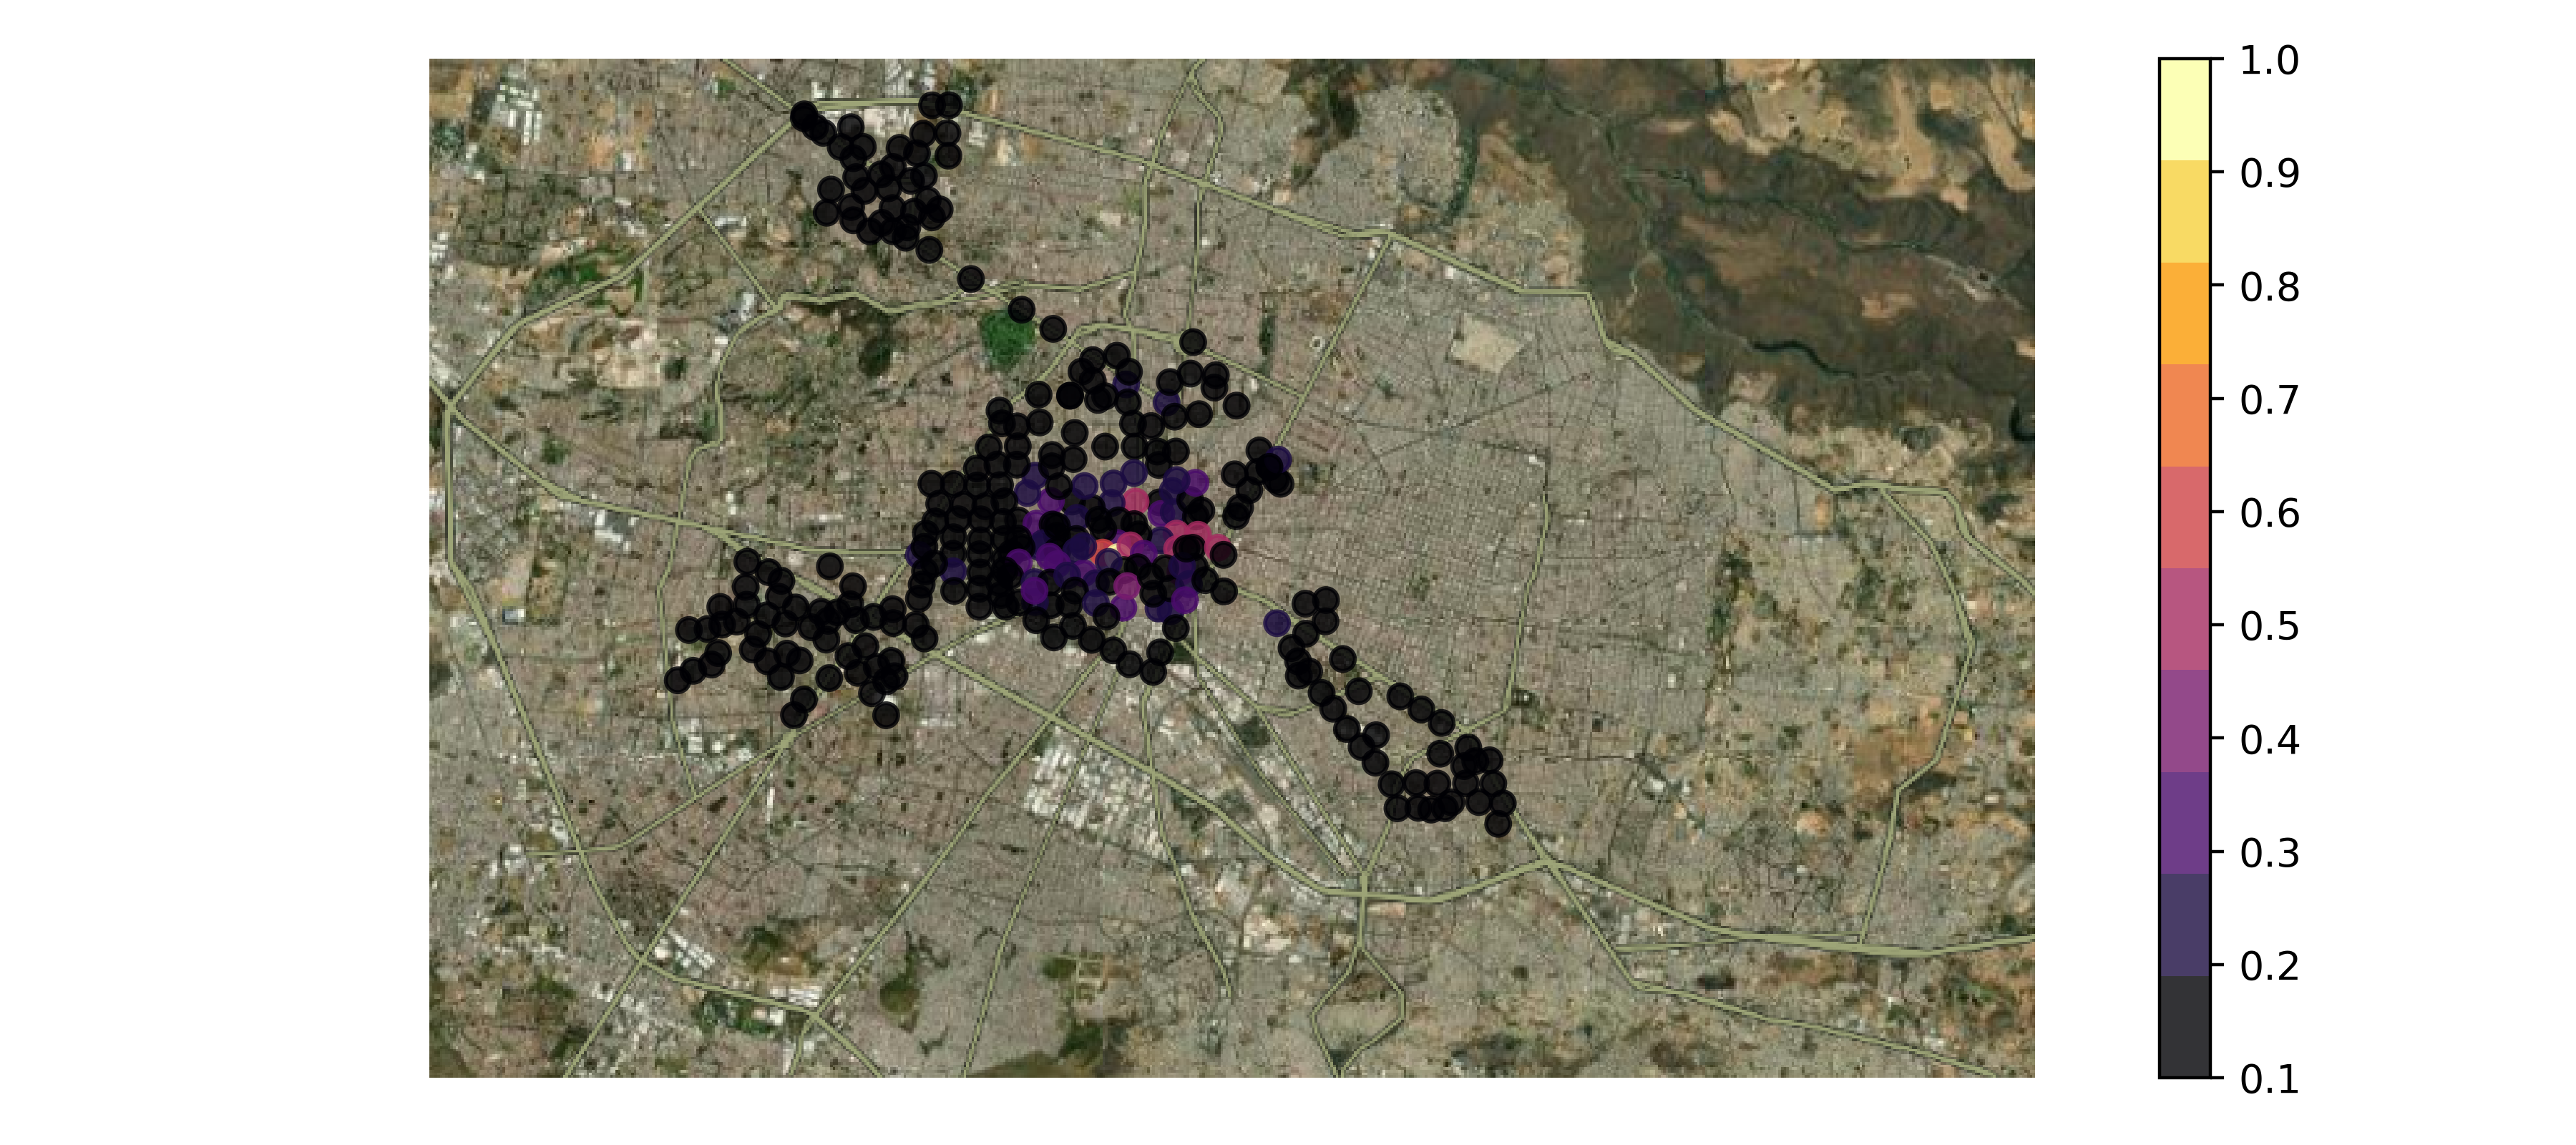
\includegraphics[width=8.2cm]{Graphics/repetition_destino.png}
        \caption{Zona metropolitana de Guadalajara.}
        \label{fig:distribution_station_all_destiny}
    \end{subfigure}
    % \hspace{0.5cm}
    \begin{subfigure}[b]{8.2cm}
        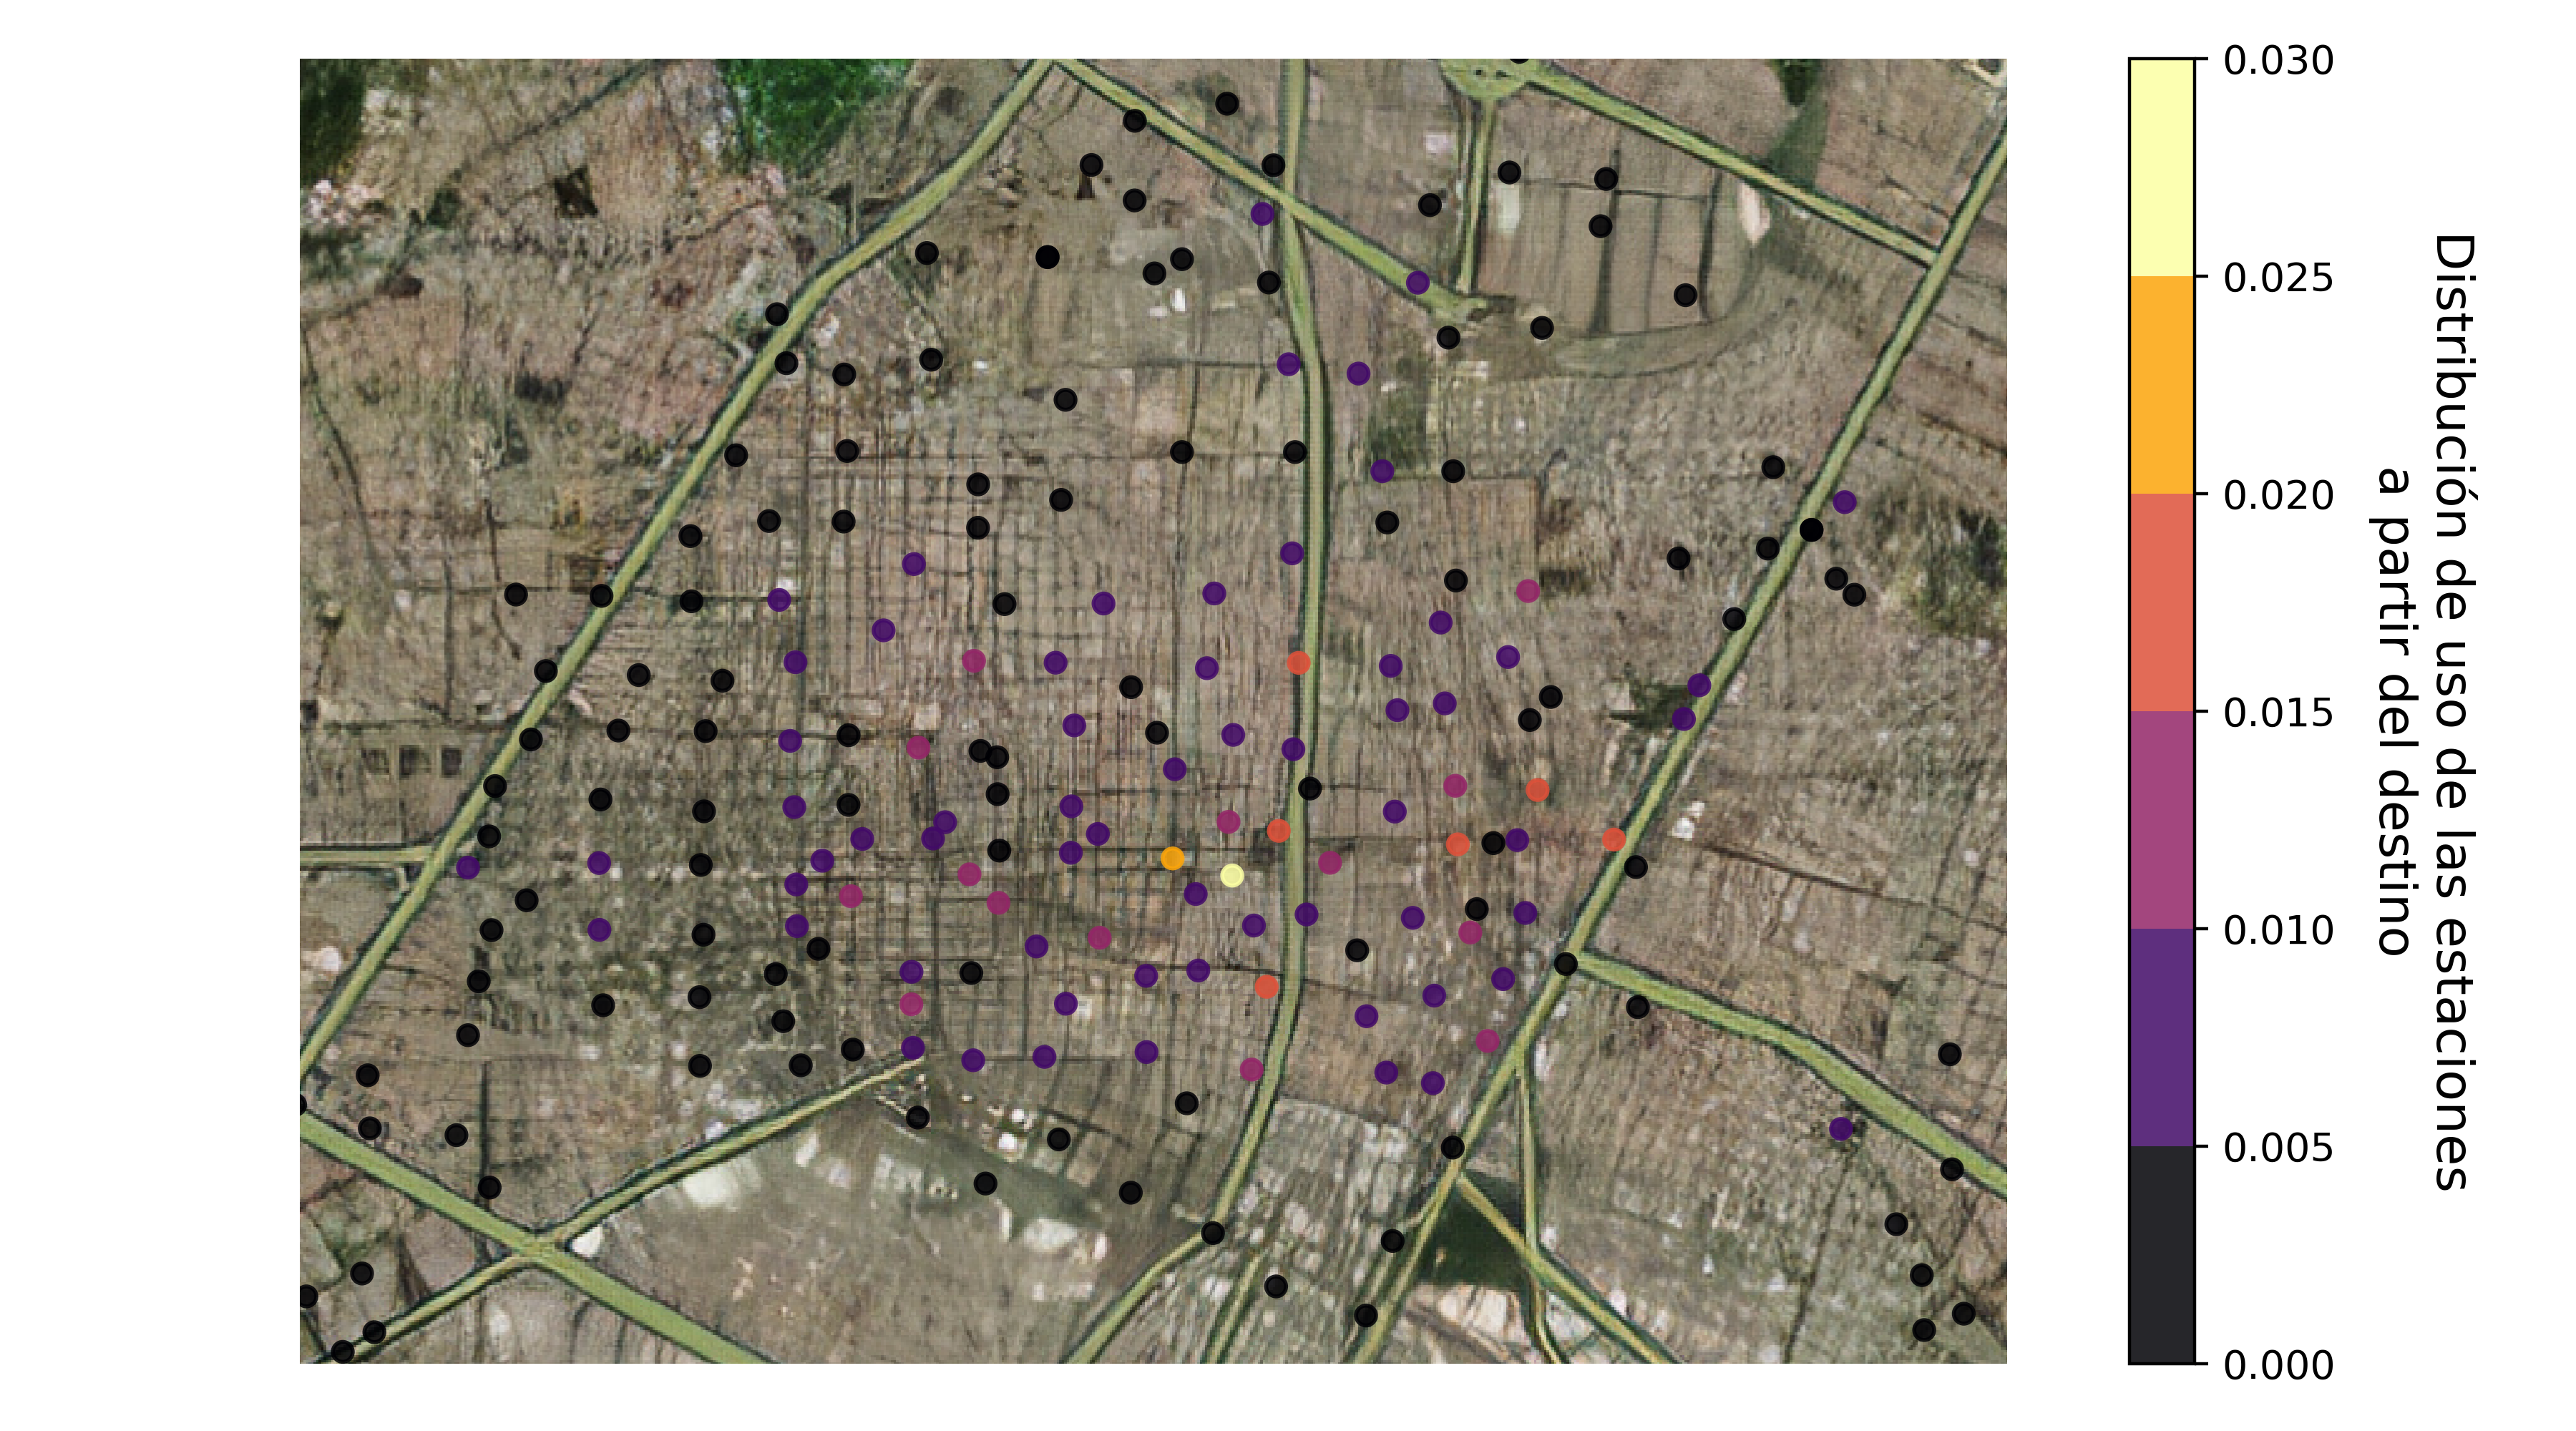
\includegraphics[width=8.2cm]{Graphics/repetition_destino_zoom.png}
        \caption{Zona de Chapultepec y Santa Tere.}
        \label{fig:distribution_station_zoom_destiny}
    \end{subfigure}
    \caption{Distribución del uso de las estaciones de MiBici como punto de destino.}
    \label{fig:distribution_destiny}
\end{figure}

